%\documentclass[11pt]{article}

\documentclass[dvipdfmx,uplatex]{jsarticle} %for headings in Japanese

 %\usepackage[margin=1in]{geometry}          
\usepackage[dvipdfmx]{graphicx}
%\usepackage{amsthm, amsmath, amssymb}
%\usepackage{setspace}\onehalfspacing
%\usepackage[loose,nice]{units} %replace "nice" by "ugly" for units in upright fractions
\graphicspath{{./img/}}

\begin{document}
\title{自主プロジェクトレポート\\
Mini Mobile Manipulator ロボット}
\author{利光泰徳}
\date{2018年1月30日}
\maketitle
\begin{center}
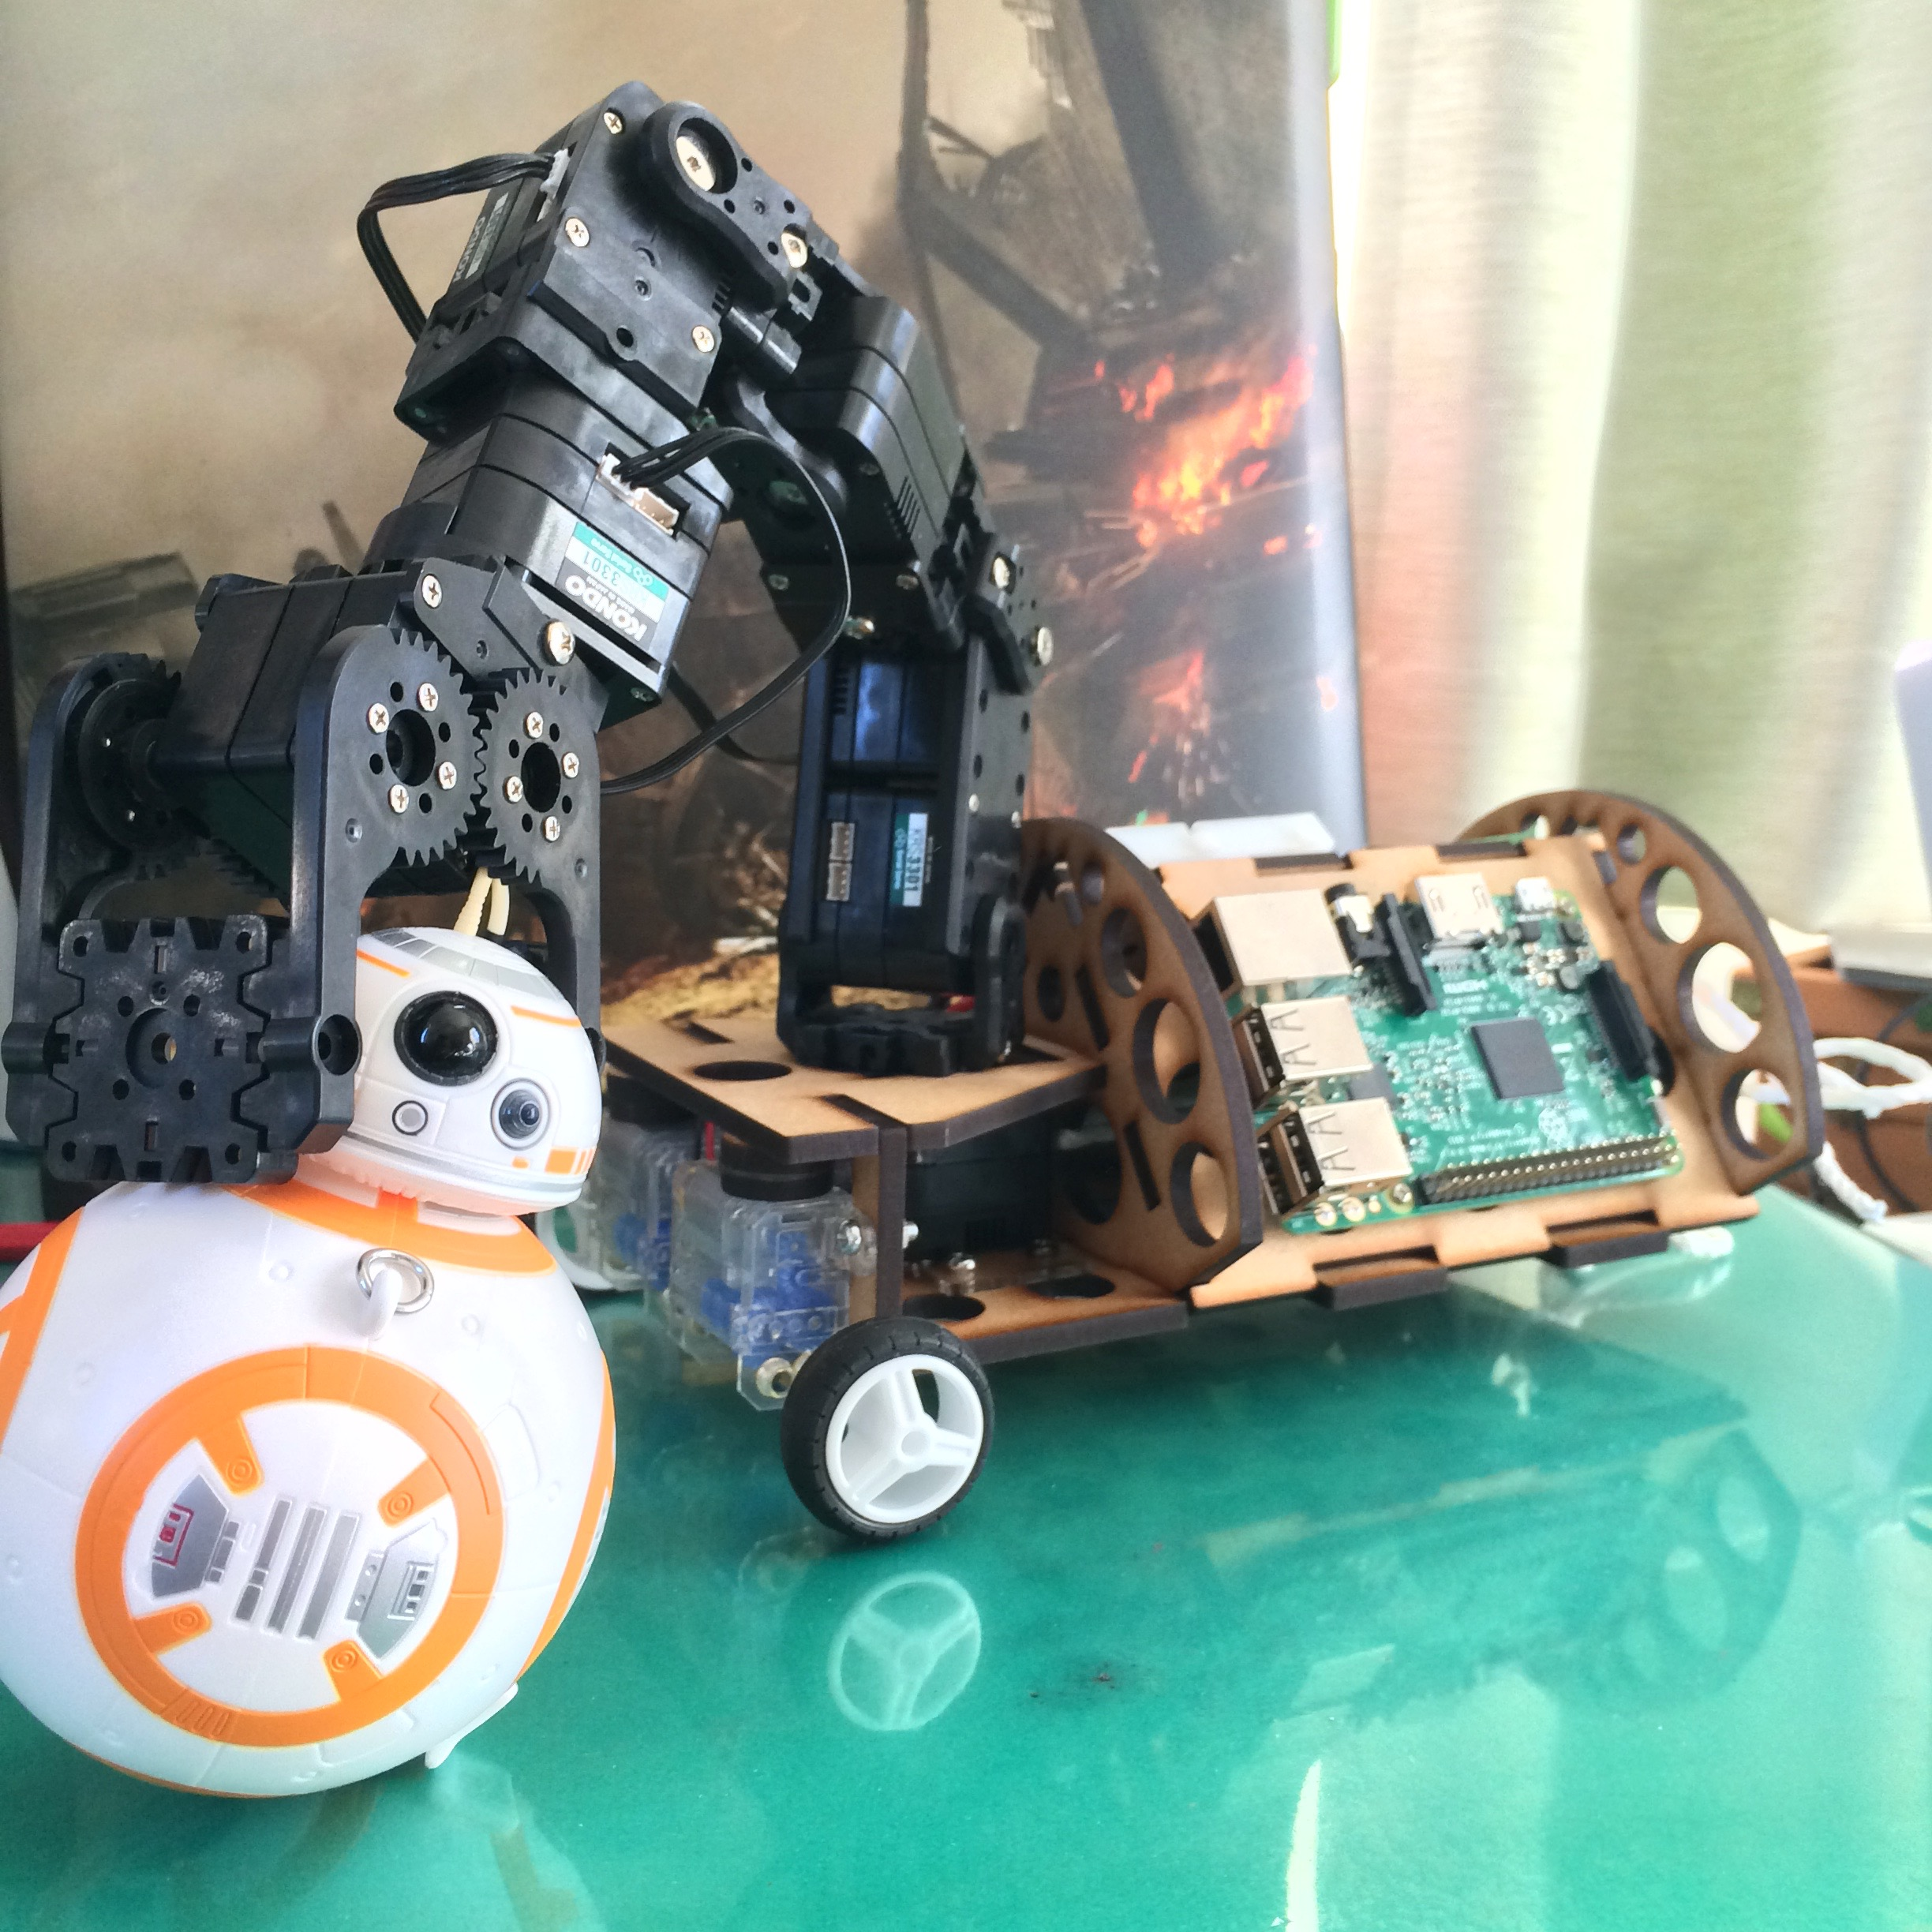
\includegraphics[width=5in]{img/model.jpg}
\end{center}
\begin{flushright}
東京大学工学部機械情報工学科3年   03-170294

レポジトリ:https://github.com/Yasu31/Mini-Mobile-Manipulator
\end{flushright}

\pagebreak

\begin{abstract}
概要です。
\end{abstract}

\section{序文}
\cite{survey_of_robots}
\cite{youbot}
\cite{low_cost_7dof}
\section{方法}
\section{結果}
\section{考察}
\section{結論}

\bibliographystyle{plain}
\bibliography{ref/citation-220942082,ref/youbot,ref/low_cost_7dof}

\end{document}